\section{The {\tt FOR} language}
\label{sec:FOR}
\begin{table}[htb]
	\begin{grammar}
		<expression> ::= 
							`nil' 
				\alt 	`cons' <expression> <expression>
				\alt 	`hd' <expression>
				\alt 	`tl' <expression>
				\alt 	<variable>

		<statement-list> ::= <statement> \alt <statement> newline <statement-list>

		<block> ::= `{' <statement-list> `}'

		<statement> ::=
							<variable> `:=' <expression>
				\alt	`if' <expression> <block> <else-block>
				\alt	`for' <variable> `in' <expression> <block>
			
				<else-block> ::= <empty> \alt `else' <block>
				
				<program> ::= <name> `read' <variable> <block> `write' <variable>
	\end{grammar}
	\caption{The \FOR syntax \label{tab:FOR-syntax}}
\end{table}

\subsection{The Elements} % (fold)
\label{sub:The Elements}
The \FOR language contains only very basic commands, but they can be combined
to implement a huge number of algorithms. As the data structure, we choose 
the humble {\tt cons} cell, that contains only a reference as the head and 
another as the tail.\footnote{An observant reader will notice that this
structure stems from the building of linked lists.}
.
\begin{figure}[htb]
	\begin{center}
		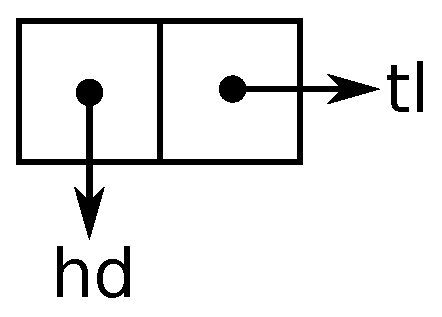
\includegraphics[height=3cm]{for/images/conscell}
	\end{center}
	\caption{The {\tt cons} cell}
\end{figure}

The expression {\tt cons e1 e2} constructs such a cell with the evaluation of
e1 in the head and the evaluation of e2 in the tail. The expression {\tt hd e1}
yields the head of the evaluation of e1 and {\tt tl e1} its tail. Since all our
current constructs need another expression, we also need a "bottom" to this
regress. We add {\tt nil} as an expression, which is distinct from any {\tt
cons e f}. We also want to refer to stored values, so an identifier (eg {\tt
X}) can also be an expression.

There are very few types of statements in \FOR, just three to be precise. The 
first is the {\em assignment} {\tt X := e}, which assigns the variable {\tt X}
the evaluation of {\tt e}. Later, when {\tt X} is used in an expression, it 
will reproduce this value. The second is the classic {\tt if} statement, that 
only executes its first block, if the expression does {\em not} return {\tt nil} 
and the else-block -- if any -- otherwise. Finally, there is the eponymous 
{\tt for} loop, that works as follows:

\begin{enumerate}
	\item On first entering the loop, the expression is evaluated and lets call 
		it $e$.
	\item If the evaluation is {\tt nil}, the loop is not evaluated anymore.
	\item Otherwise the block is evaluated with the value of the head of $e$.
	\item Then this procedure is run again with the tail of $e$.
\end{enumerate}

\subsection{\FOR computability}
\lineofthought{
	\begin{itemize}
		\item number of steps computable $\rightarrow$ function that takes this 
			may steps is computable.
	\end{itemize}
}
\subsection{Non-\FOR computability}
\lineofthought{
	\begin{itemize}
		\item Ackermann
		\item Self-interpretation
	\end{itemize}
}
